
\section{Partioparaati 28.4.}

\vspace*{-0.64cm}
\begin{multicols}{2}

	\begin{center}
		\noindent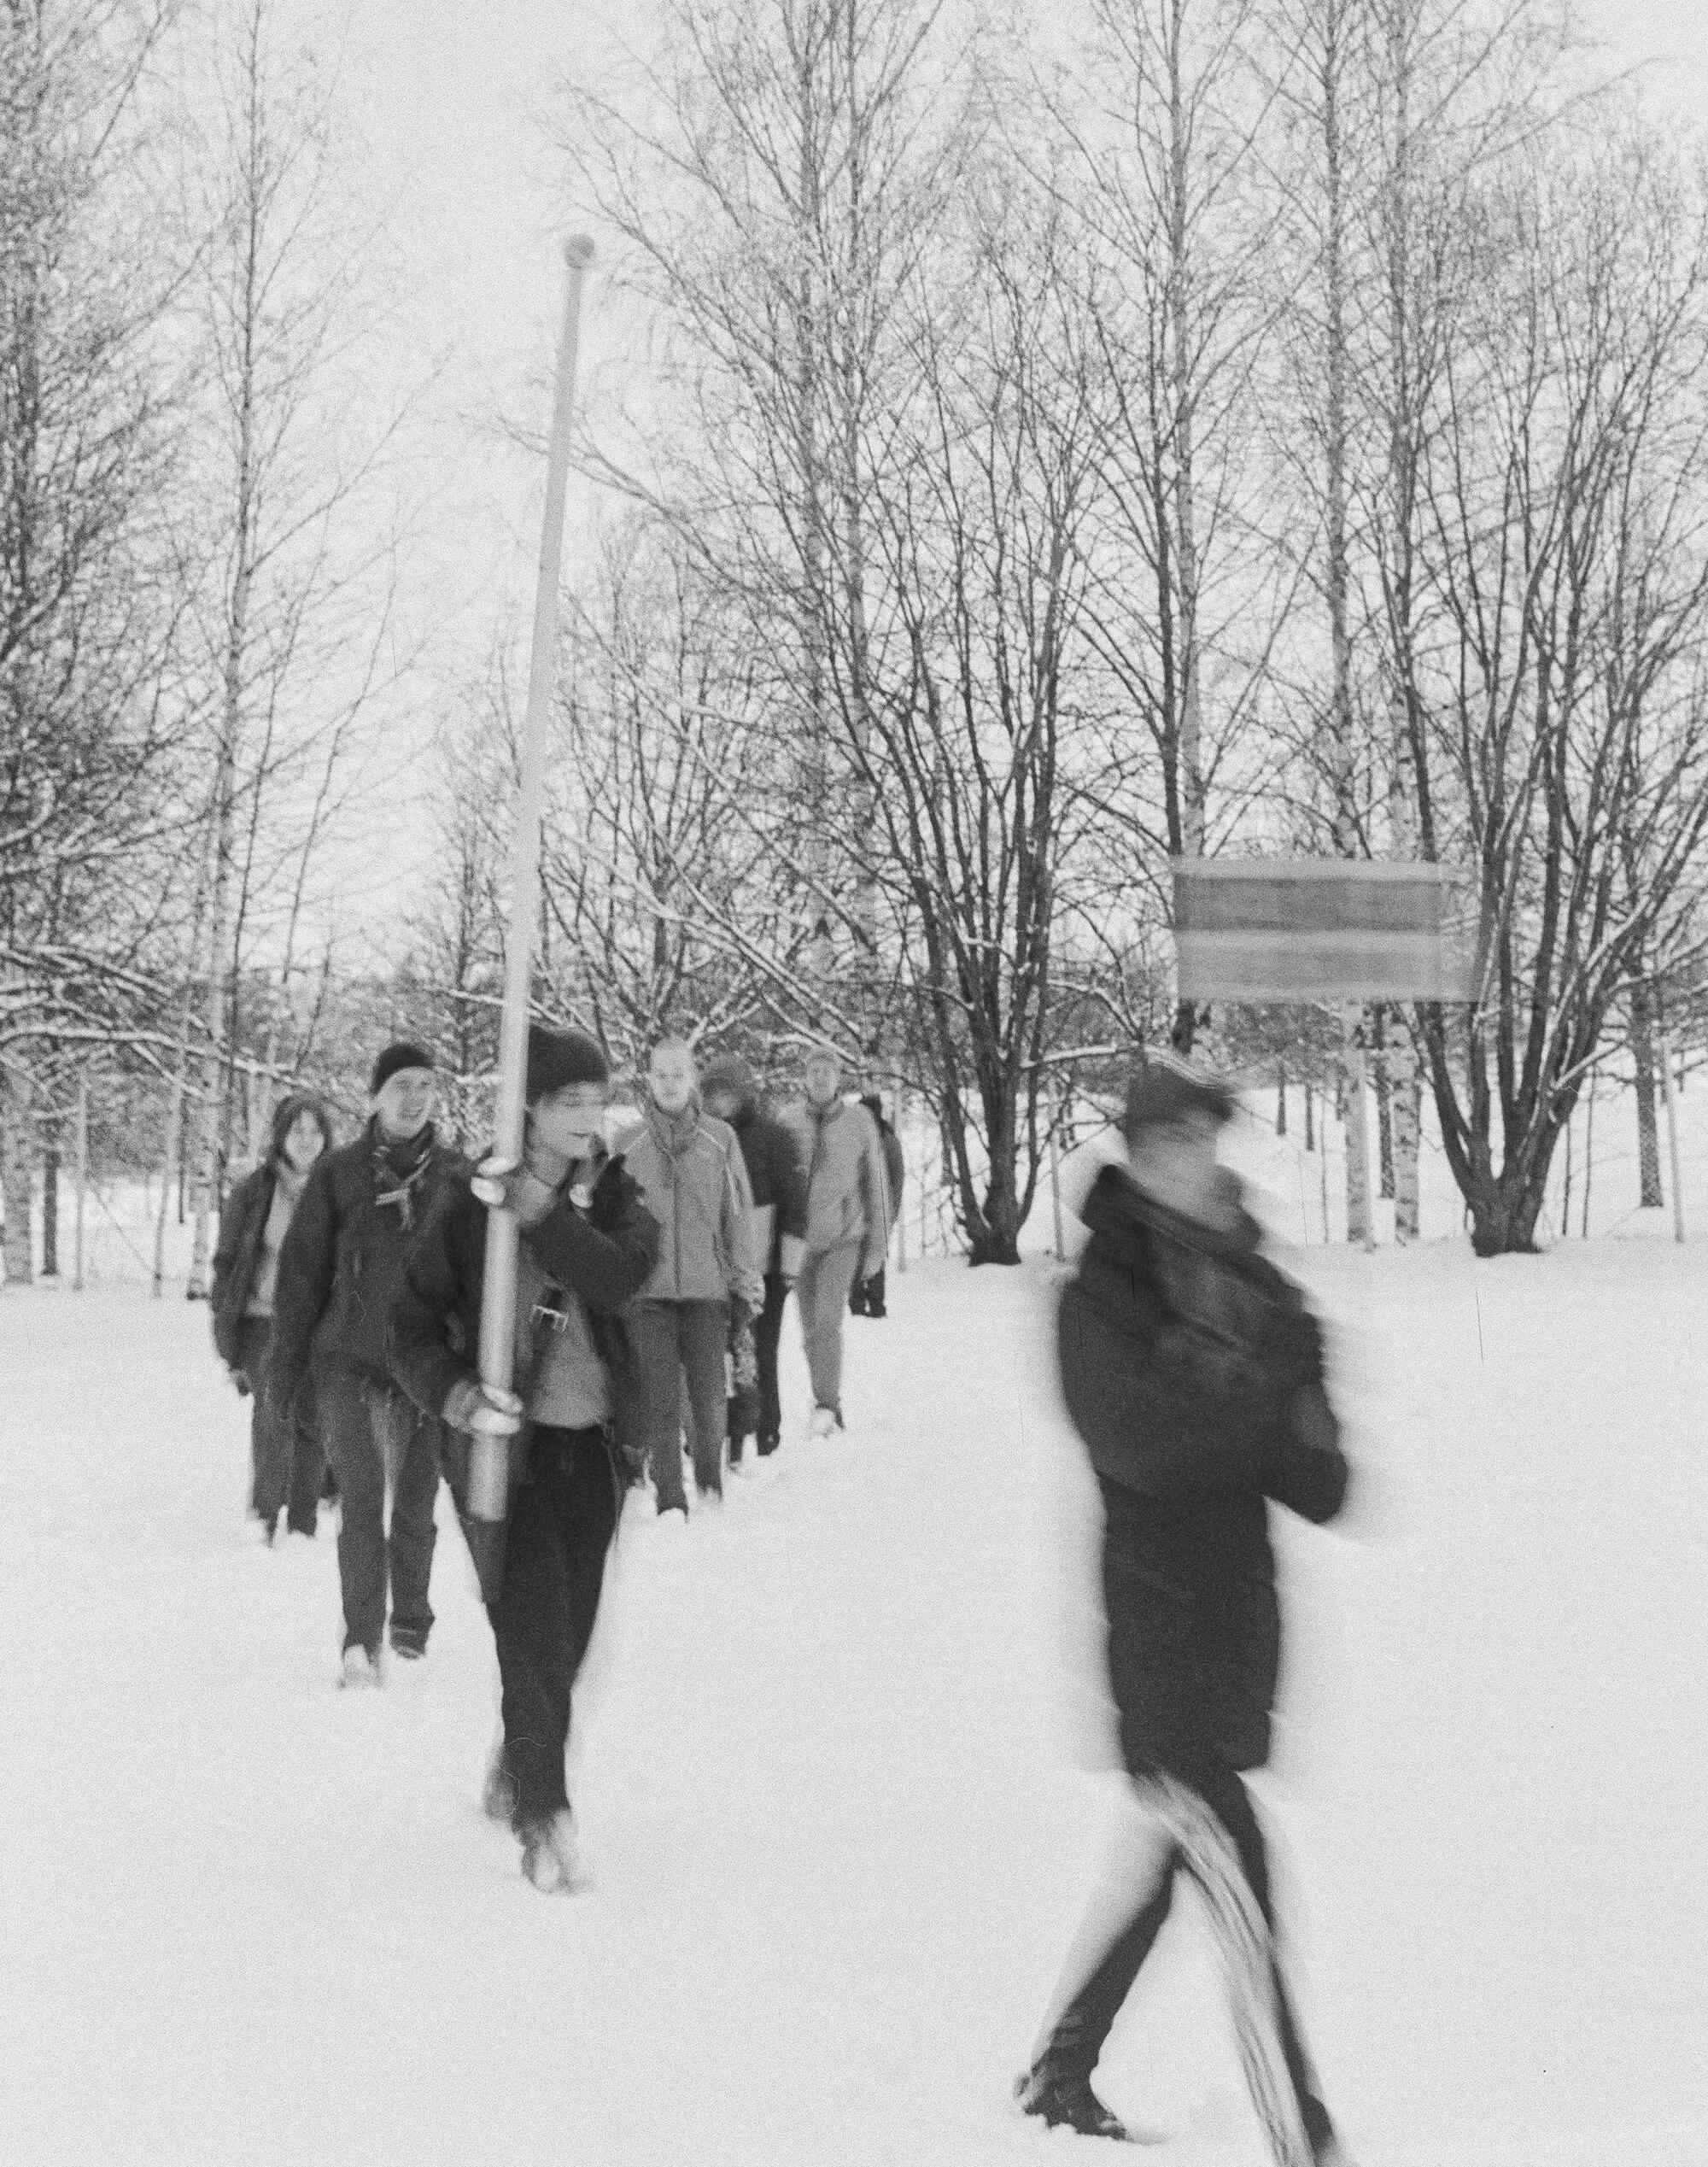
\includegraphics[width=0.85\linewidth]{assets/paraati1}
	\end{center}

	\vspace*{-0.32cm}
	\small KuRu:n paraatiosasto harjoiteli \mbox{paraati}protokollan
	viikkokokouksessa, vielä talvisella säällä \ldots

	\columnbreak

	\begin{center}
		\noindent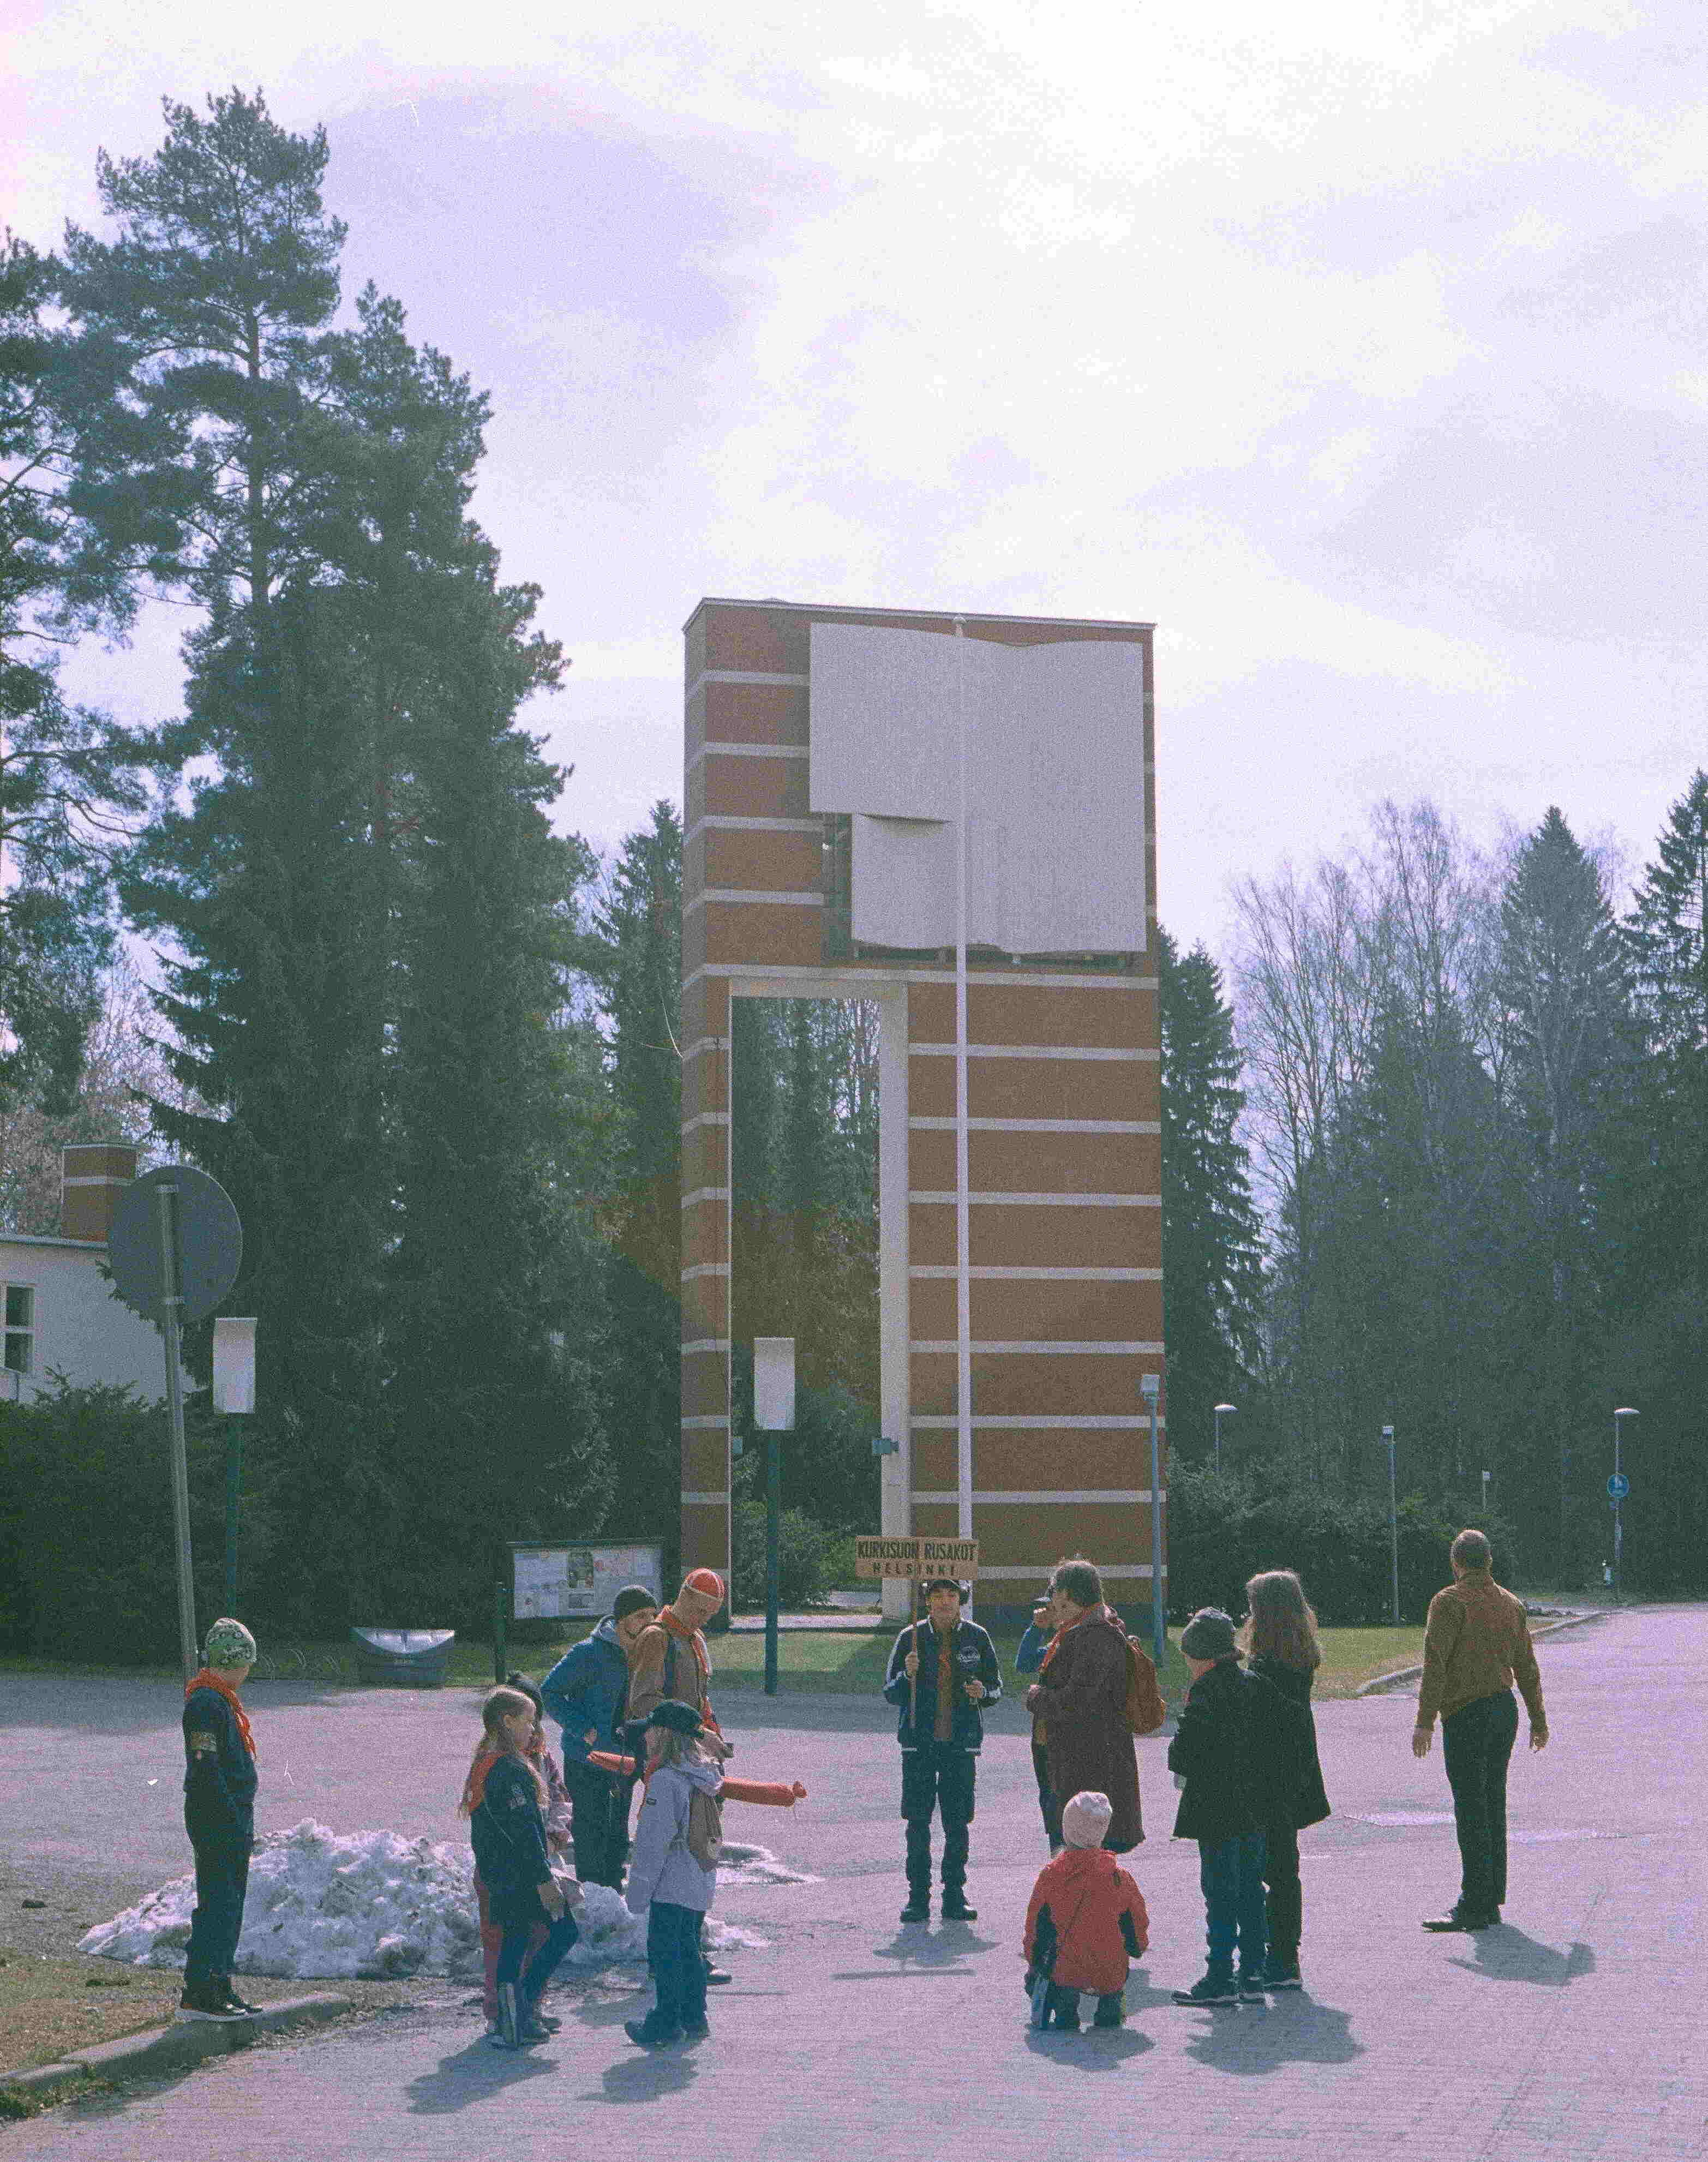
\includegraphics[width=0.85\linewidth]{assets/paraati2}
	\end{center}

	\vspace*{-0.32cm}
	\ldots ja pari päivää myöhemmin, kokoontui keväisessä kelissä ja matkusti kohti keskustan.

\end{multicols}
\begin{multicols}{2}

	\begin{center}
		\noindent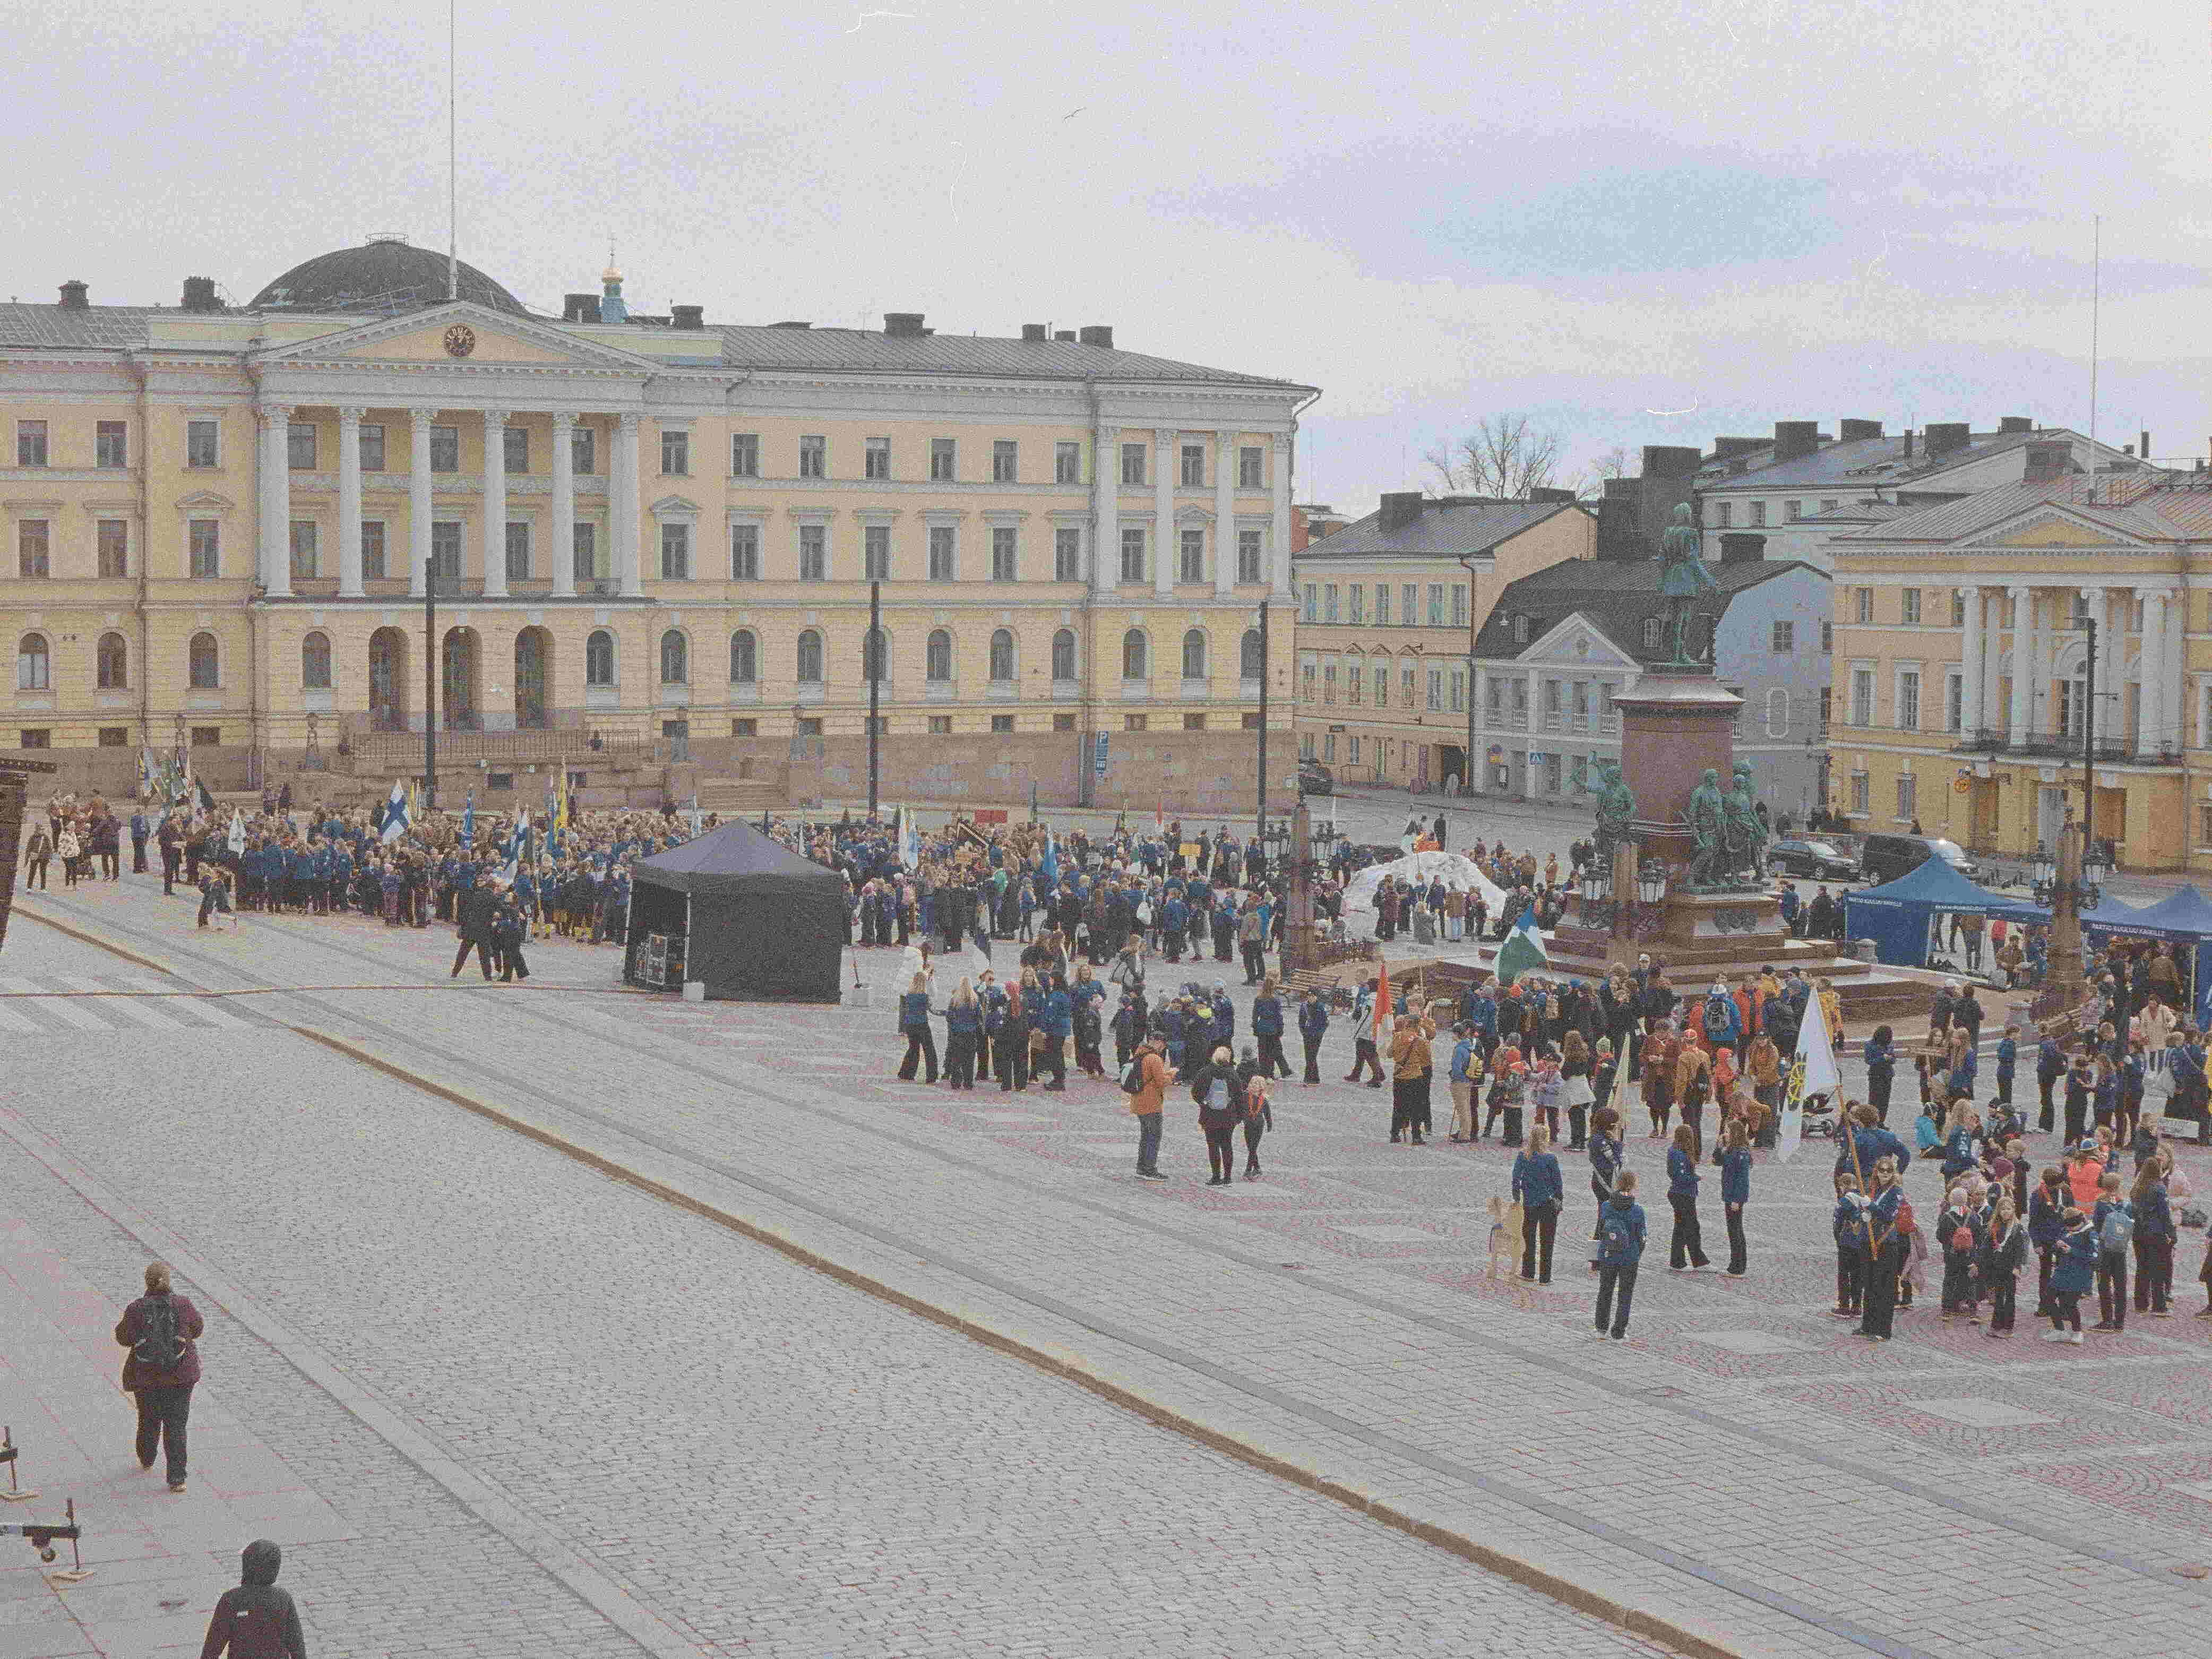
\includegraphics[width=0.85\linewidth]{assets/paraati4}
	\end{center}

	\vspace*{-0.16cm}
	\small Senaatintorilla löytyi yli kaksi tuhatta partiolaista Helsingistä, Espoosta, Vantaasta ja Kauniaisesta. Siellä marsittiin, nautitiin musiikista ja ajoittain auringosta.

	Paraatin päätteeksi, KuRu:n osasto sai vielä maistuva lounas läheisessä \mbox{pitseriassa}!

	\columnbreak

	\begin{center}
		\noindent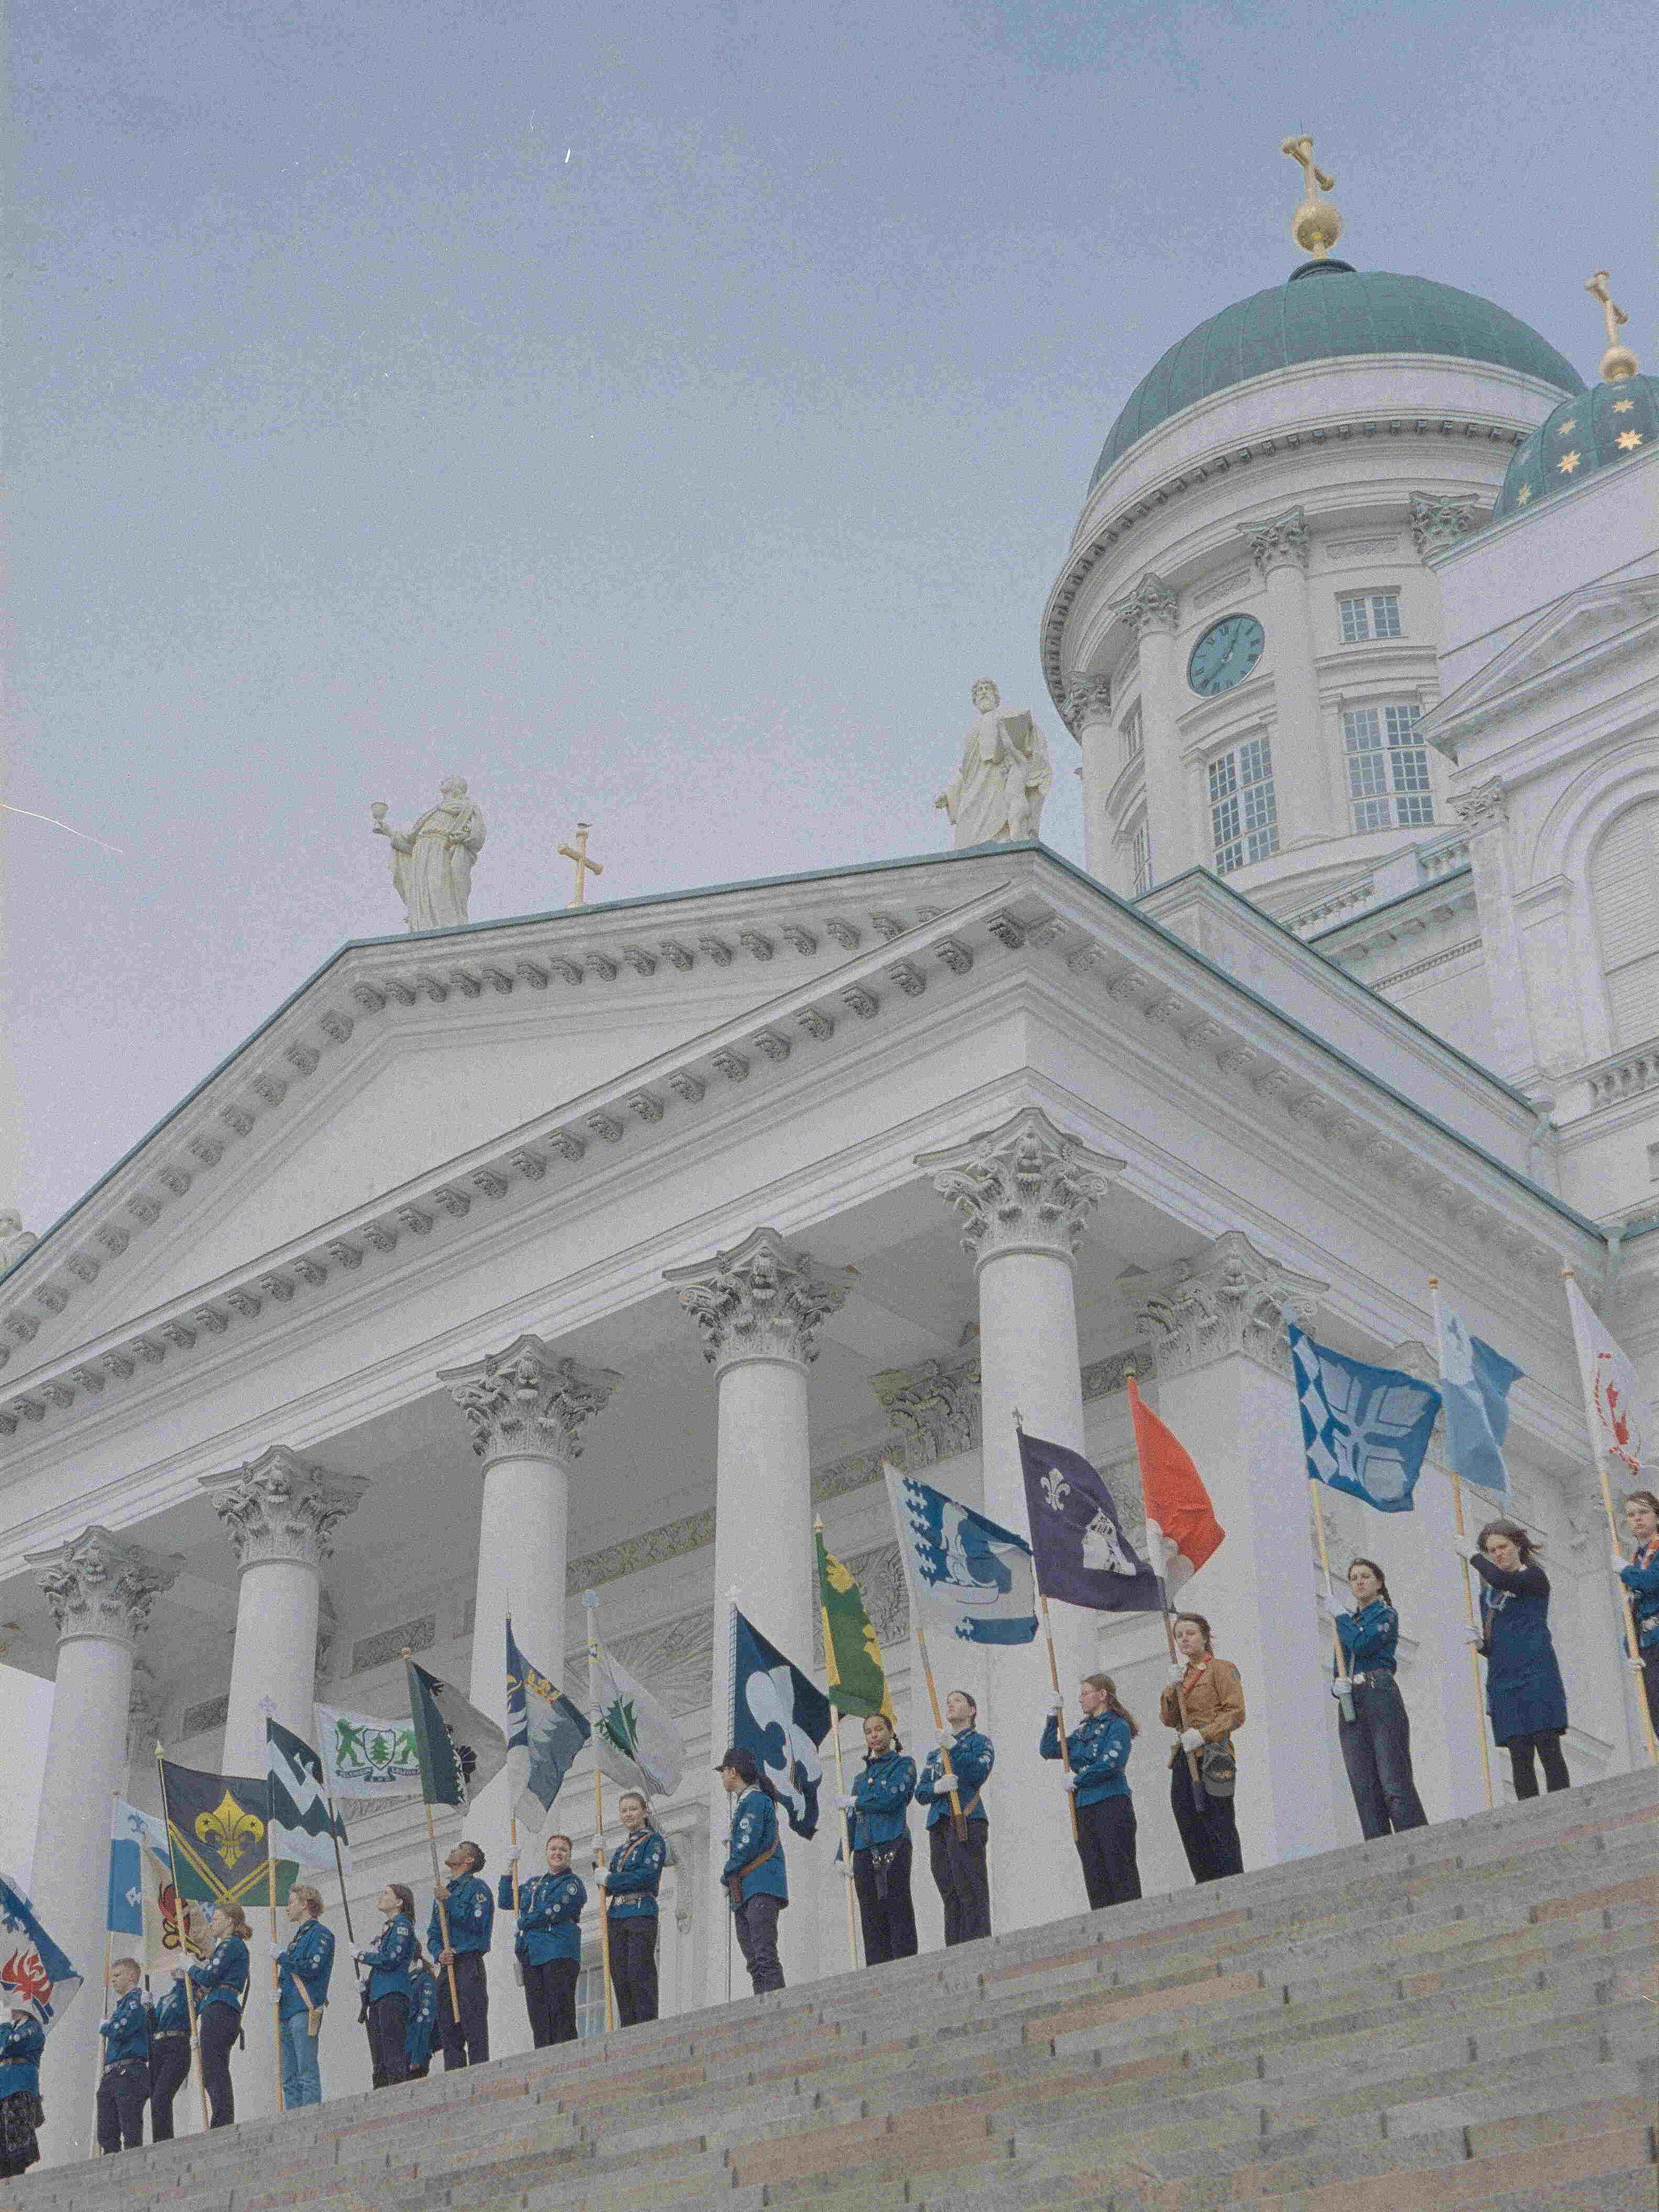
\includegraphics[width=0.85\linewidth]{assets/paraati3}
	\end{center}


\end{multicols}

% \vspace*{-0.32cm}

\medskip
\noindent\null\hfill Tanguy Gérôme
